\chapter{Introducción}

Uno de los puntos más débiles en la seguridad de toda organización ha sido las contraseñas. Cuando el usuario dispone de absoluto control sobre la decisión de cómo debe ser ésta, las contraseñas tienden a ser muy débiles ante ataques de diccionario. La solución a este problema reside en el uso de políticas de contraseña que exijan unos mínimos de fortaleza (uso de minúsculas y mayúsculas, números y símbolos). Estas políticas se pueden controlar informáticamente obligando al usuario poner contraseñas de calidad.

Por otra parte la potencia de las CPUs se ha incrementando, lo que ha supuesto la necesidad de mejorar los sistemas criptográficos para hacerlos más resistentes a todo tipo de ataques. En el caso concreto de las funciones resumen este fortalecimiento se ha materializado de dos formas distintas:

\begin{itemize}
	\item Se ha incrementado el número de bits del resumen para disminuir la posibilidad de colisiones.
	\item Se procura mejorar la técnica de generación del resumen para garantizar que los resúmenes sean lo más aleatorios posibles, utilizando procesos que impidan determinar el mensaje a partir del resumen y que garanticen estar normalmente\footnote{Si los resúmenes generados no tuviesen una distribución normal esto supondría que habría grupos de resúmenes y facilitaría ataques contra éstos pues sería más fácil determinar de dónde podrían proceder.} distribuidos. 
\end{itemize}

Estas mejoras ha ido esquivando uno de los problemas más importantes que han tenido las funciones resumen: el incremento de la potencia de las CPUs permite realizar ataques de fuerza bruta en tiempos asumibles.

El incremento de la potencia de las CPUs se ha visto restringido por la capacidad de integración de transistores en un microprocesador y el diseño interno del mismo. Si tomamos la Ley de Moore ésta dice que el número de transistores en un microprocesador tiende a duplicarse cada 18 meses. Esto nos permite planificar qué capacidad de cómputo podría tener un CPU en el futuro de cara a evitar ataques de fuerza bruta. De todos modos, el número de transistores es solo una parte de la capacidad de una CPU ya que su estructura interna afecta también de forma muy clara. Esto se debe a la forma que tiene de organizar la ejecución de una aplicación, la calidad del predictor de saltos, etc.

Al mismo tiempo a la mejora de las CPUs, se ha ido produciendo una importante mejora en las GPUs. Estos procesadores de propósito específico han visto su potencia incrementada muy rápidamente gracias a sus diseños más sencillos (se utilizan específicamente para cálculo matemático) y a su gran capacidad de paralelización (una NVIDIA Tesla puede disponer de hasta 970 núcleos) como puede verse en la Figura \ref{fig:GPUvsCPU}. Desde hace algún tiempo las tarjetas gráficas permiten cargar pequeños trozos de códigos denominados \emph{shaders} (éstos códigos se utilizan como filtros para efectos 3D) y esta técnica a desembocado en permitir la carga de códigos de usuario más genéricos.

\begin{figure}
	\centering
	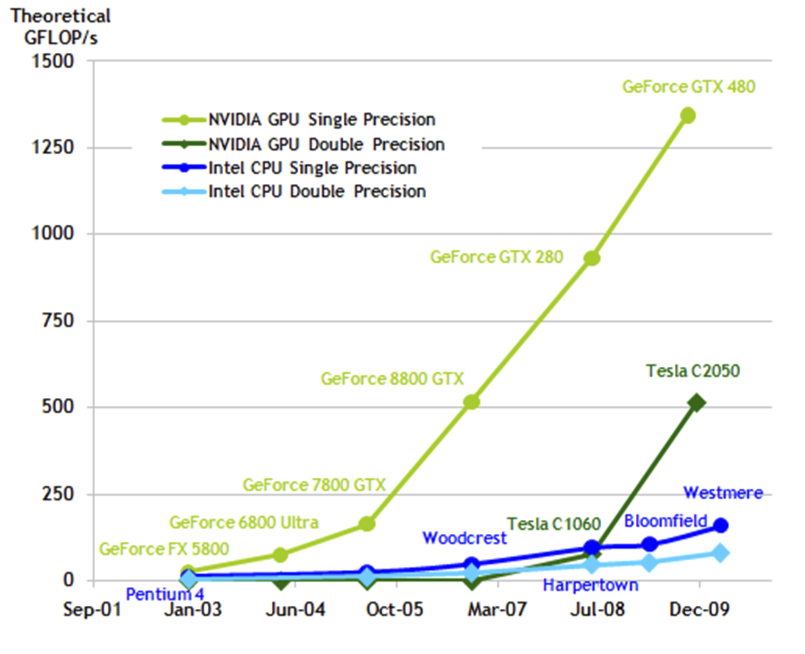
\includegraphics[width=0.7\textwidth]{evolucion-gpu.png}
	\caption{Comparativa de la evolución de los GFlops de las GPUs frente a las CPUs\cite{nvidia:cuda_c_programming_guide}}\label{fig:GPUvsCPU}
\end{figure}

La principal razón por la que el uso de GPU para computación se ha convertido en algo de interés es la publicación de APIs como CUDA y OpenCl que nos permiten aprovechar las capacidades de las actuales tarjetas gráficas para realizar cálculos y operaciones muy costosas en tiempo de CPU de forma más rápida. Además, permiten un alto grado de paralelismo, lo que puede resultar beneficioso para el desarrollo de ciertos tipos de programas.

En la actualizadad, mientras con una CPU se podía conseguir hasta 80 millones de claves MD5 por segundo (aplicando muchas optimizaciones a nivel de lenguaje ensamblador), una GPU potente puede alcanzar hasta cerca de los 2.000 millones de resúmenes por segundo. Esto es, una GPU es hasta 250 veces más rápida que la CPU para este tipo de cálculos, propiciado, principalmente, por su mayor capacidad de paralelización.

Si consideramos el hecho de que en la actualidad casi todos los nuevos equipos que se venden en el mercado disponen de aceleradoras gráficas y que es muy fácil crear una red de ordenadores zombis se debe considerar la mejora de los mecanismos de contraseña una prioridad por parte de las organizaciones. Por este motivo es importante disponer de herramientas que permitan comprobar la fortaleza de las contraseñas y evaluar la dificultad de realizar ataques a los distintos algoritmos de resumen existentes y en experimentación.

\section{Objetivos}
El presente proyecto final de carrera nace con el objetivo de aprovechar las nuevas arquitecturas gráficas en el entorno de la auditoría de seguridad informática. Igualmente se ha pretendido utilizar un modelo distribuido para mejorar la escalabilidad del sistema y así disponer de una herramienta potente que pueda ser ampliada según la necesidad del momento.

\section{Estructura del documento}

